\documentclass{article}

%Aus dem LaTex Template der Universit�t Stuttgart
%------------------------------------------------
\usepackage[utf8]{inputenc}
\usepackage[T1]{fontenc}
\usepackage[sfdefault]{ClearSans} %% option 'sfdefault' activates Clear Sans as the default text font
\usepackage{cmap}
\usepackage[ngerman]{babel}
\usepackage{graphicx}
\usepackage[pdftex,hyperref,dvipsnames]{xcolor}
\usepackage{listings}
\usepackage[a4paper,lmargin={2cm},rmargin={2cm},tmargin={3.5cm},bmargin = {2.5cm},headheight = {4cm}]{geometry}
\usepackage{amsmath,amssymb,amstext,amsthm}
\usepackage[lined,algonl,boxed]{algorithm2e}
\usepackage{tikz}
\usepackage{hyperref}
\usepackage{url}
\usepackage[inline]{enumitem} % Erm�glicht �ndern der enum Item Zahlen
\usepackage[headsepline]{scrpage2} 
\usepackage{algorithmic} % F�r Pseudocode
\usepackage{ marvosym } % f�r Pfeil(e)
\usepackage{booktabs} % F�r die sch�neren Booktabs-Tabellen
\usepackage{tikz}
\usepackage{pdfpages}
\usepackage{blindtext}
\usepackage{scrextend}
\usepackage{pdfpages}
\usepackage{natbib} % Yannis hat das importiert; TODO: nachfragen, zu was das gut ist
\pagestyle{scrheadings} 
\usetikzlibrary{automata,positioning}

\begin{document}
	%%% Vorgegebenes Deckblatt %%%
	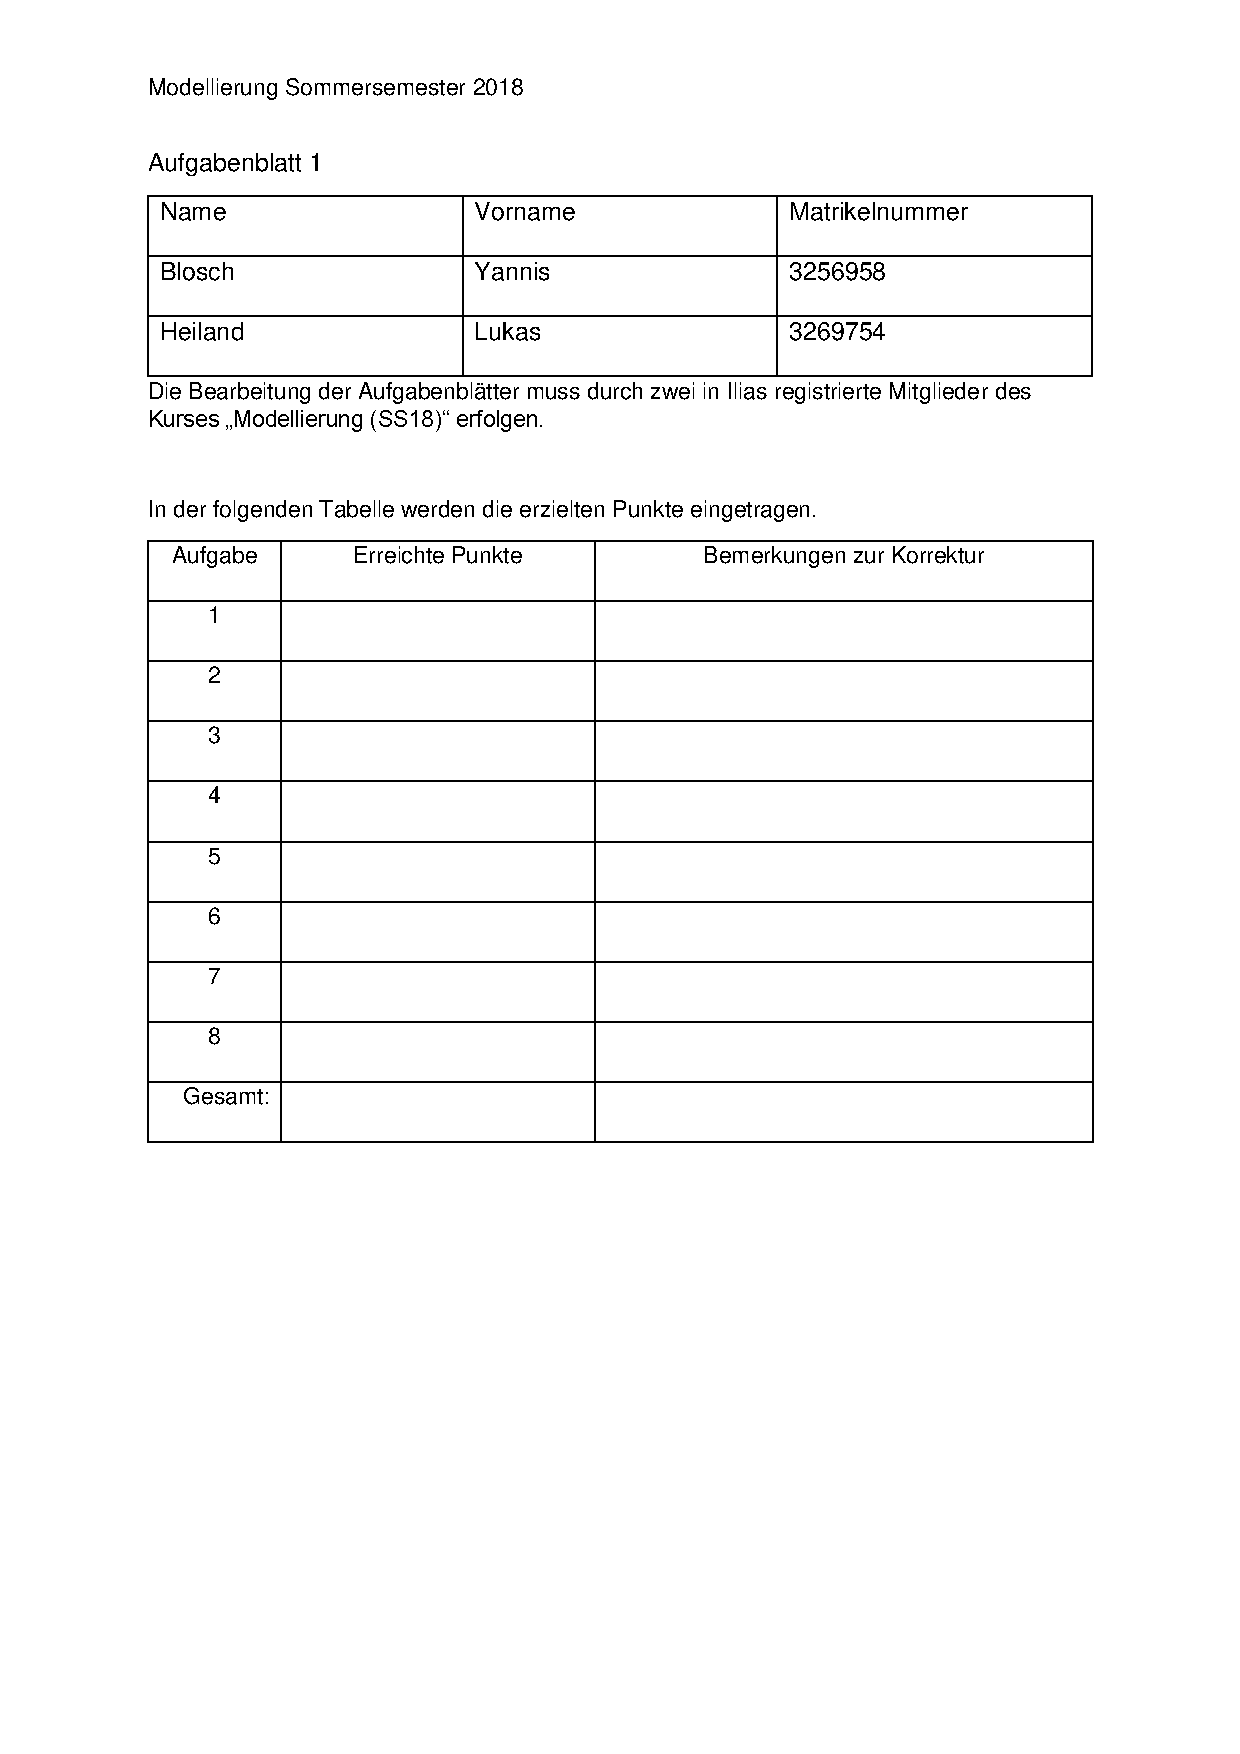
\includepdf{deckblatt.pdf}
	
	%%% format and header %%%
	% Counter für das Blatt und die Aufgabennummer.
% Ersetze die Nummer des Übungsblattes und die Nummer der Aufgabe
% den Anforderungen entsprechend.
% Beachte:
% \setcounter{countername}{number}: Legt den Wert des Counters fest
% \stepcounter{countername}: Erhöht den Wert des Counters um 1.
\newcounter{sheetnr}
\setcounter{sheetnr}{1} % Nummer des Übungsblattes
\newcounter{exnum}
\setcounter{exnum}{1} % Nummer der Aufgabe

% Befehl für die Aufgabentitel
\newcommand{\exercise}[1]{\section*{Aufgabe \theexnum\stepcounter{exnum} #1}} % Befehl für Aufgabentitel

% Formatierung der Kopfzeile
% \ohead: Setzt rechten Teil der Kopfzeile mit
% Namen und Matrikelnummern aller Bearbeiter
\ohead{Yannis Blosch (3256958)\\
Lukas Heiland (3269754)}
% \chead{} kann mittleren Kopfzeilen Teil sezten
% \ihead: Setzt linken Teil der Kopfzeile mit
% Modulnamen, Semester und Übungsblattnummer
\ihead{Modellierung\\
Sommersemester 2018\\
Blatt \thesheetnr}
	
	%%%%%%%%%%%%%%%%%%%%%%%%%%%%%%
	%%%%%%% actual content %%%%%%%
	%%%%%%%%%%%%%%%%%%%%%%%%%%%%%%
	
	\section*{Aufgabe 4.1}
		% relationale Algebra: Datum aller Darlehen über >5.000€
		\paragraph*{a.}
			$\pi_{Datum}(\rho_{(d\_kredithoehe>5.000)} darlehen)$
			
		% rel. Algebra: IDs aller Konten die ein Darl. über >20.000€ haben und KOntaktperson in Berlin
		\paragraph*{b.}
			% alle Mitarbeiter aus Berlin
			$Q_1 \leftarrow \rho_{a\_ort = 'Berlin'}(mitarbeiter \underset{m\_adresse = a\_id}{\bowtie} adresse)$ \\[1.2em]
			
			% alle Konten mit Kontaktperson in Berlin
			$Q_2 \leftarrow \pi_{b\_id}(bankkonto \underset{b\_kontaktperson = m\_id}{\bowtie} Q_1)$
			\\[1.2em]
			
			% alle Darlehen mit kontaktperson in Berlin und > 20.000
			$\pi_{d\_bankkonto}(\rho_{d\_kredithoehe > 20.000}(darlehen \underset{d\_bankkonto = b\_id}{\bowtie} Q_2))$\\
			
			
		% SQL-query: Name,Alter,Anzahl Kredite,PLZ aller Kunden absteigend nach Alter sortiert
		\paragraph*{c}.\\
			%%%
			\textbf{SELECT} k\_name, k\_alter, k\_kredite, adresse.a\_plz as plz\\
			\textbf{FROM} kunde, adresse\\
			\textbf{WHERE} kunde.k\_adresse = adresse.a\_id\\
			\textbf{SORT BY} k\_alter \textbf{DESCENDING}
			
		% Geben Sie eine Anfrage in SQL-Notation an, die für jeden Mitarbeiter den Namen und die Anzahl der Bankkonten, bei denen er als Kontaktperson fungiert und deren Guthaben niedriger als 5000 ist, ausgibt. Es sollen nur Mitarbeiter ausgegeben werden, die insgesamt bei weniger als 50 Bankkonten Kontaktpersonen sind.
		\paragraph*{d}.\\
			TODO
		
		% SQL-query: Name,Alter aller Kunden, die mind. 1 Darl. haben, dessen Höhe > Durchschnittskredithöhe ist (ohne Duplikate -> DISTINCT)
		\paragraph*{e.}
			TODO
		
		% SQL: immer wenn in einer Adresse "Stuttgart" vorkommt, soll der Ort in "Stuttgart" geändert werden. z.B.: Stuttgart-Vaihingen -> Stuttgart, PenisStuttgart -> Stuttgart
		\paragraph*{f.}
			TODO
	
		\pagebreak
	
	\section*{Aufgabe 4.2}
		% Gegeben ist die Datenbank aus Aufgabe 1, Einträge: s. Blatt. Zusätzlich wird folgender Trigger erstellt:
		% CREATE TRIGGER T1
			% AFTER INSERT ON darlehen
			% REFERENCING NEW ROW AS r
			% FOR EACH ROW
			% UPDATE bankkonto
			% SET b_guthaben=b_guthaben + r.d_kredithoehe
			% WHERE b_inhaber=r.d_kunde;
		% Geben Sie an, ob die Anweisung korrekt/nicht korrekt ist (mit Erklärung!)
		
		
		
	\section*{Aufgabe 4.3}
		% Zeigen Sie mit Hilfe der Armstrong-Axiome, dass die abgeleiteten Regeln (union, decomposition, pseudotransitivity) ebenfalls gelten. Geben Sie für jeden Schritt an, welche Axiome Sie benutzt haben.
		\paragraph*{union}:\\
			$\alpha \rightarrow \beta$,	$\alpha \rightarrow \gamma$ \hspace*{25mm} (gegeben)\\
			0. $\alpha \rightarrow \alpha \alpha$ \hspace*{31mm} (gilt)\\
			1. $\alpha \alpha \rightarrow \alpha \beta$ \hspace*{29mm} (augmentation der ersten gegebenen)\\
			2. $\alpha \beta \rightarrow \alpha \gamma$ \hspace*{29mm} (augmentation der zweiten gegebenen)\\
			3. $\alpha \rightarrow \alpha \beta$ \hspace*{31mm} (transitivity von 0. und 1.)\\
			4. $\alpha \rightarrow \beta \gamma$ \hspace*{31mm} (transitivity von 1. und 2.)
			
		\paragraph*{decomposition}:\\
			1. $\alpha \rightarrow \beta \gamma$ \hspace*{31mm} (gegeben)\\
			2. $\beta \gamma \rightarrow \beta$ \hspace*{31mm} (reflexivity, $\beta \subseteq \beta\gamma$)\\
			3. $\alpha \rightarrow \beta$ \hspace*{33mm} (transitivity der oberen zwei Zeilen)\\
			analog für $\alpha \rightarrow \gamma$
		
		\paragraph*{pseudotransitivity}:\\
			$\alpha \rightarrow \beta, \beta\gamma \rightarrow \delta$ \hspace*{25mm} (gegeben)\\
			1. $ \alpha\gamma \rightarrow \beta\gamma $ \hspace*{29mm} (augmentation der ersten gegebenen mit $\gamma$)
			2. $\alpha \gamma \rightarrow \delta$ \hspace*{31mm} (transititvity der zweiten gegebenen und 1.)\\
			
			
		
		
	\section*{Aufgabe 4.4}
		\paragraph*{CLOSURE($\{ F \}, Z\backslash\{F \longrightarrow G\}$})\\
		result $=$ \{F\}\\
		
			\{F,C,D\} \hspace*{42mm} wegen $F \rightarrow CD$\\
			
			\{F,C,D,A\} \hspace*{39mm} wegen $D \rightarrow A$\\
			
			\{F,C,D,A,G,H\} \hspace*{32mm} wegen $AC \rightarrow GH$\\
			
			\hspace*{11mm}\textbf{\vdots}\\[1.2em]
			$G \in CLOSURE(\{F\}, Z \backslash \{F \longrightarrow G\})$\\
			$\Rightarrow F \rightarrow G$ ist redundante funktionale Abhängigkeit
	
		\paragraph*{CLOSURE($\{H\}, Z \backslash \{H \rightarrow B\}$})\\
		H steht auf keiner linken Seite der funktionalen Abh"angigkeiten in der Menge Z\\
		$\rightarrow B \notin CLOSURE(\{H\}, Z \backslash \{H \rightarrow B\})$\\ $\Rightarrow H \rightarrow B$ ist keine redundante funktionale Abhängigkeit
		
	
	
\end{document}